\section{Angular Distribution}

\begin{frame}{Impact Matrix}
    	\vspace{-0.05\textheight}
    \begin{overlayarea}{\textwidth}{0.1\textheight}
	\centering
	\textbf{11~h. acquisition long at $\mathbf{\sim 4\ 10^{4}}$~pps}
	%\vspace{0.05\textheight}
	\end{overlayarea}
	\begin{columns}
		\begin{column}{0.5\textwidth}
			\begin{overlayarea}{\textwidth}{\textheight}
				\centering
				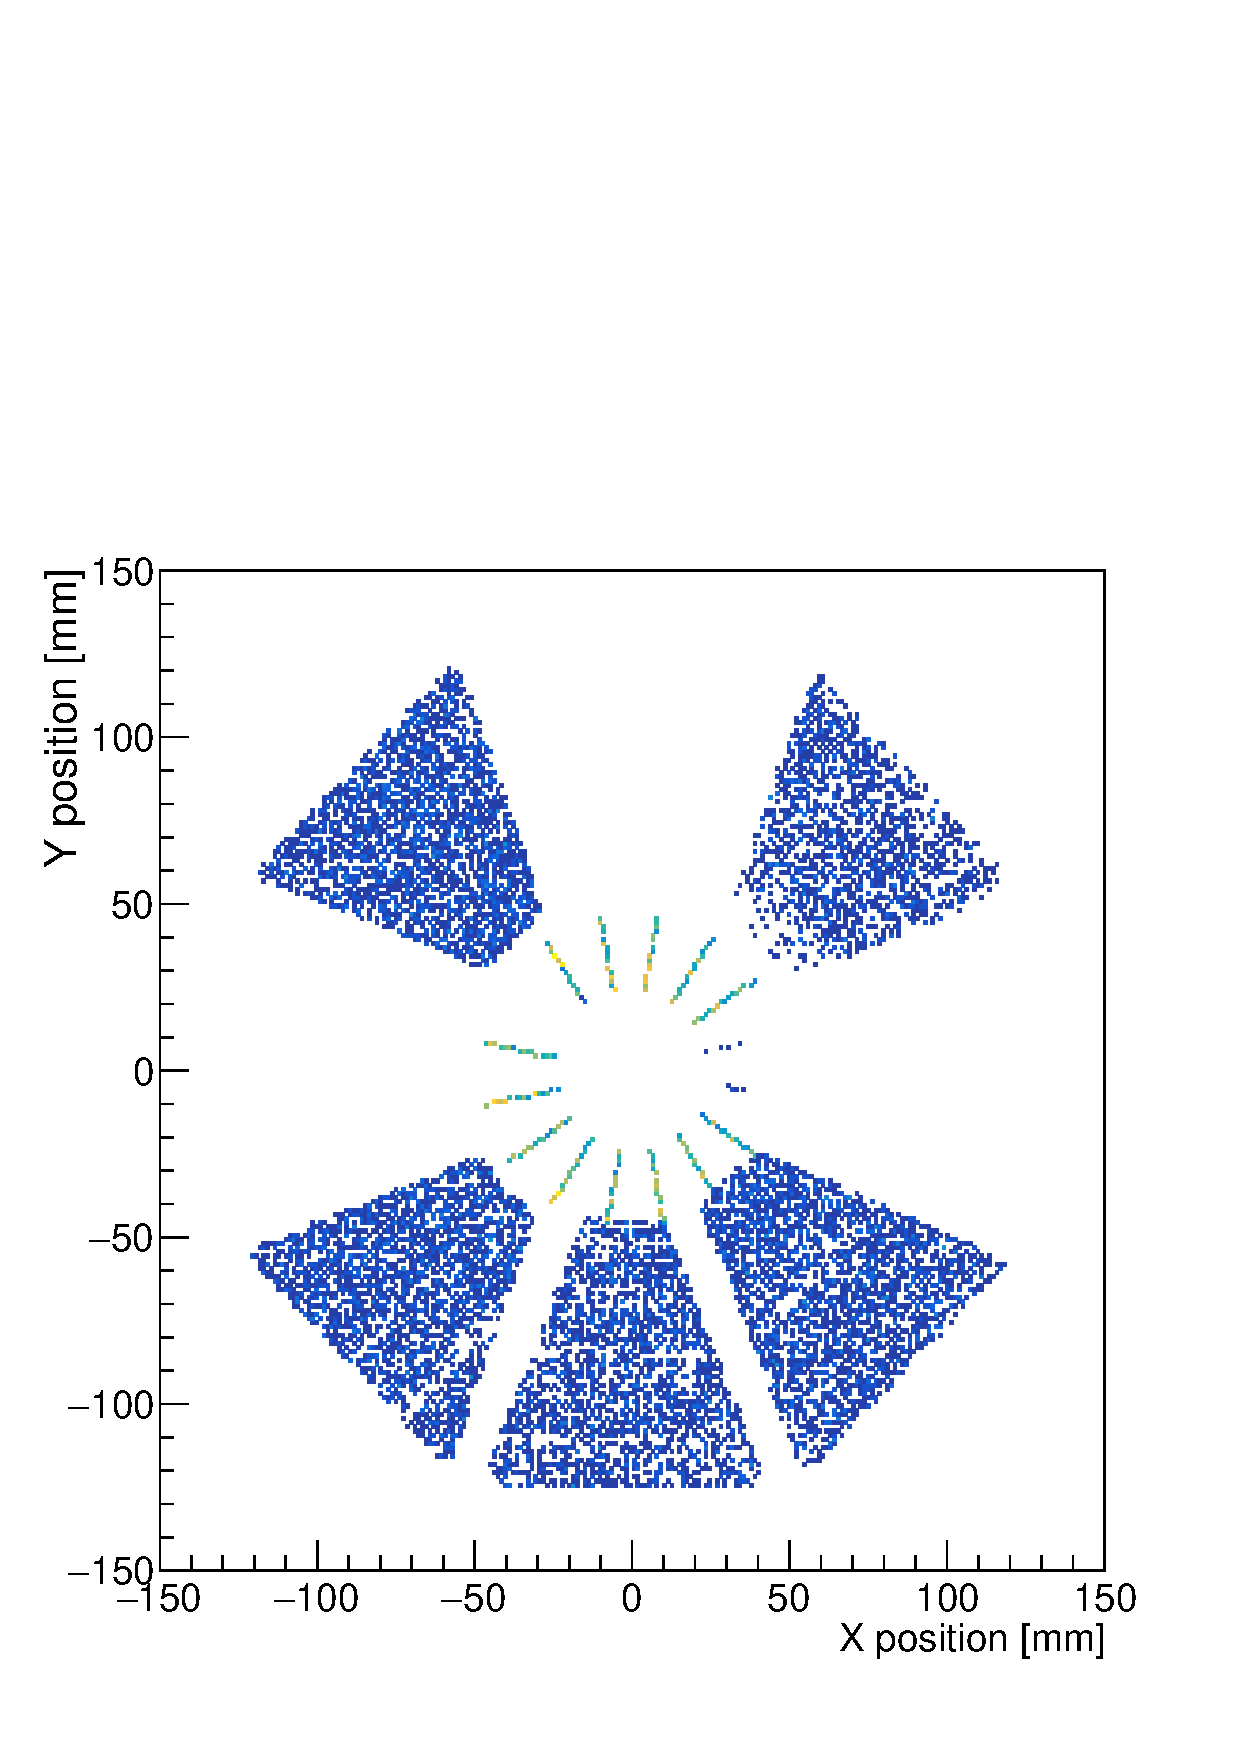
\includegraphics[width=\textwidth]{MGimpact}
			\end{overlayarea}
		\end{column}
		\begin{column}{0.5\textwidth}
			\begin{overlayarea}{\textwidth}{\textheight}
				\centering       
				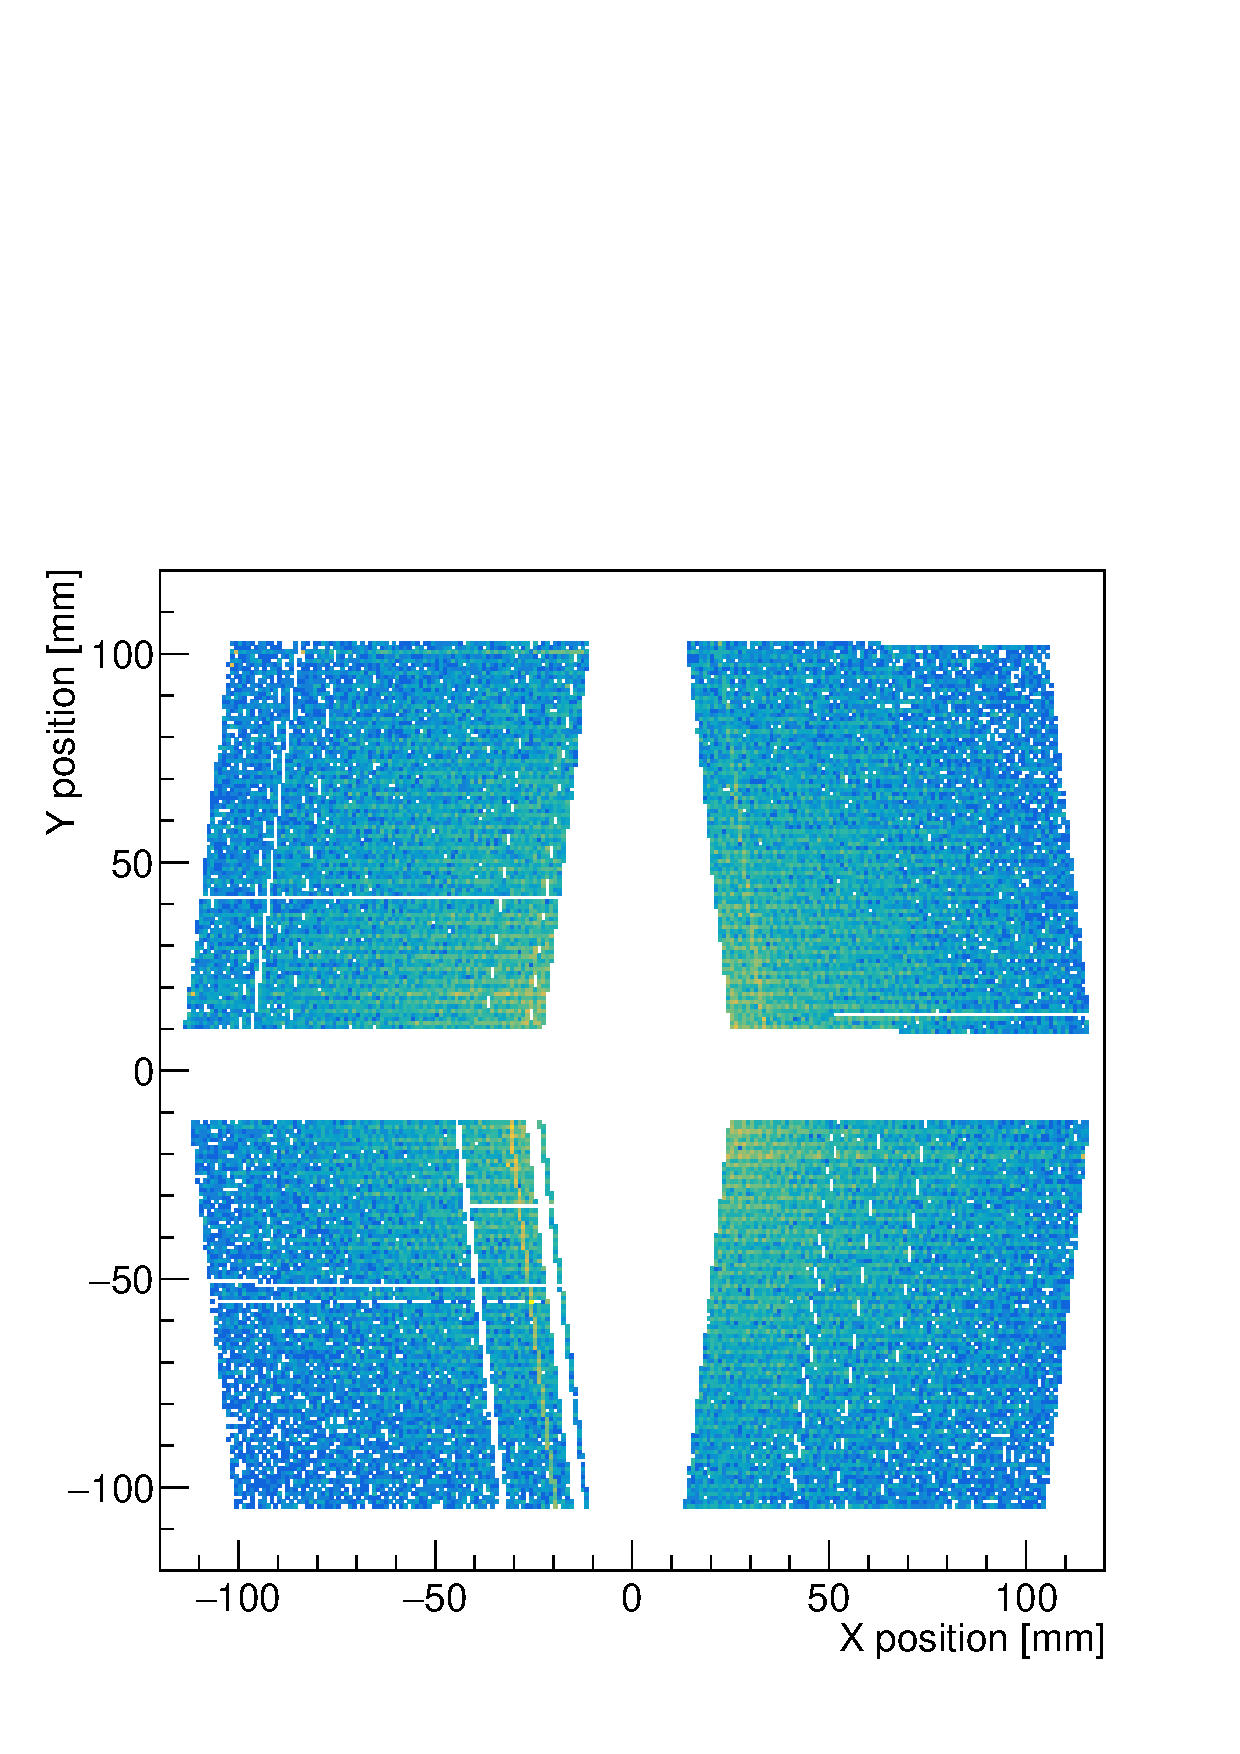
\includegraphics[width=\textwidth]{MMimpact}\\
		    \end{overlayarea}	
		\end{column}
	\end{columns}
\end{frame}

\begin{frame}{Kinematic Lines}
    	\vspace{-0.05\textheight}
    \begin{overlayarea}{\textwidth}{0.1\textheight}
	%\vspace{0.001\textheight}
	%\only<1>{No clear kinematic lines on MUST2}
	\end{overlayarea}	
	\vspace{-0.05\textheight}
	\begin{columns}
		\begin{column}{0.43\textwidth}
			\begin{overlayarea}{\textwidth}{\textheight}
				\centering
				%\vspace{0.02\textheight}
				\only<1>{\footnotesize No clear kinematic lines on MUST2\\
				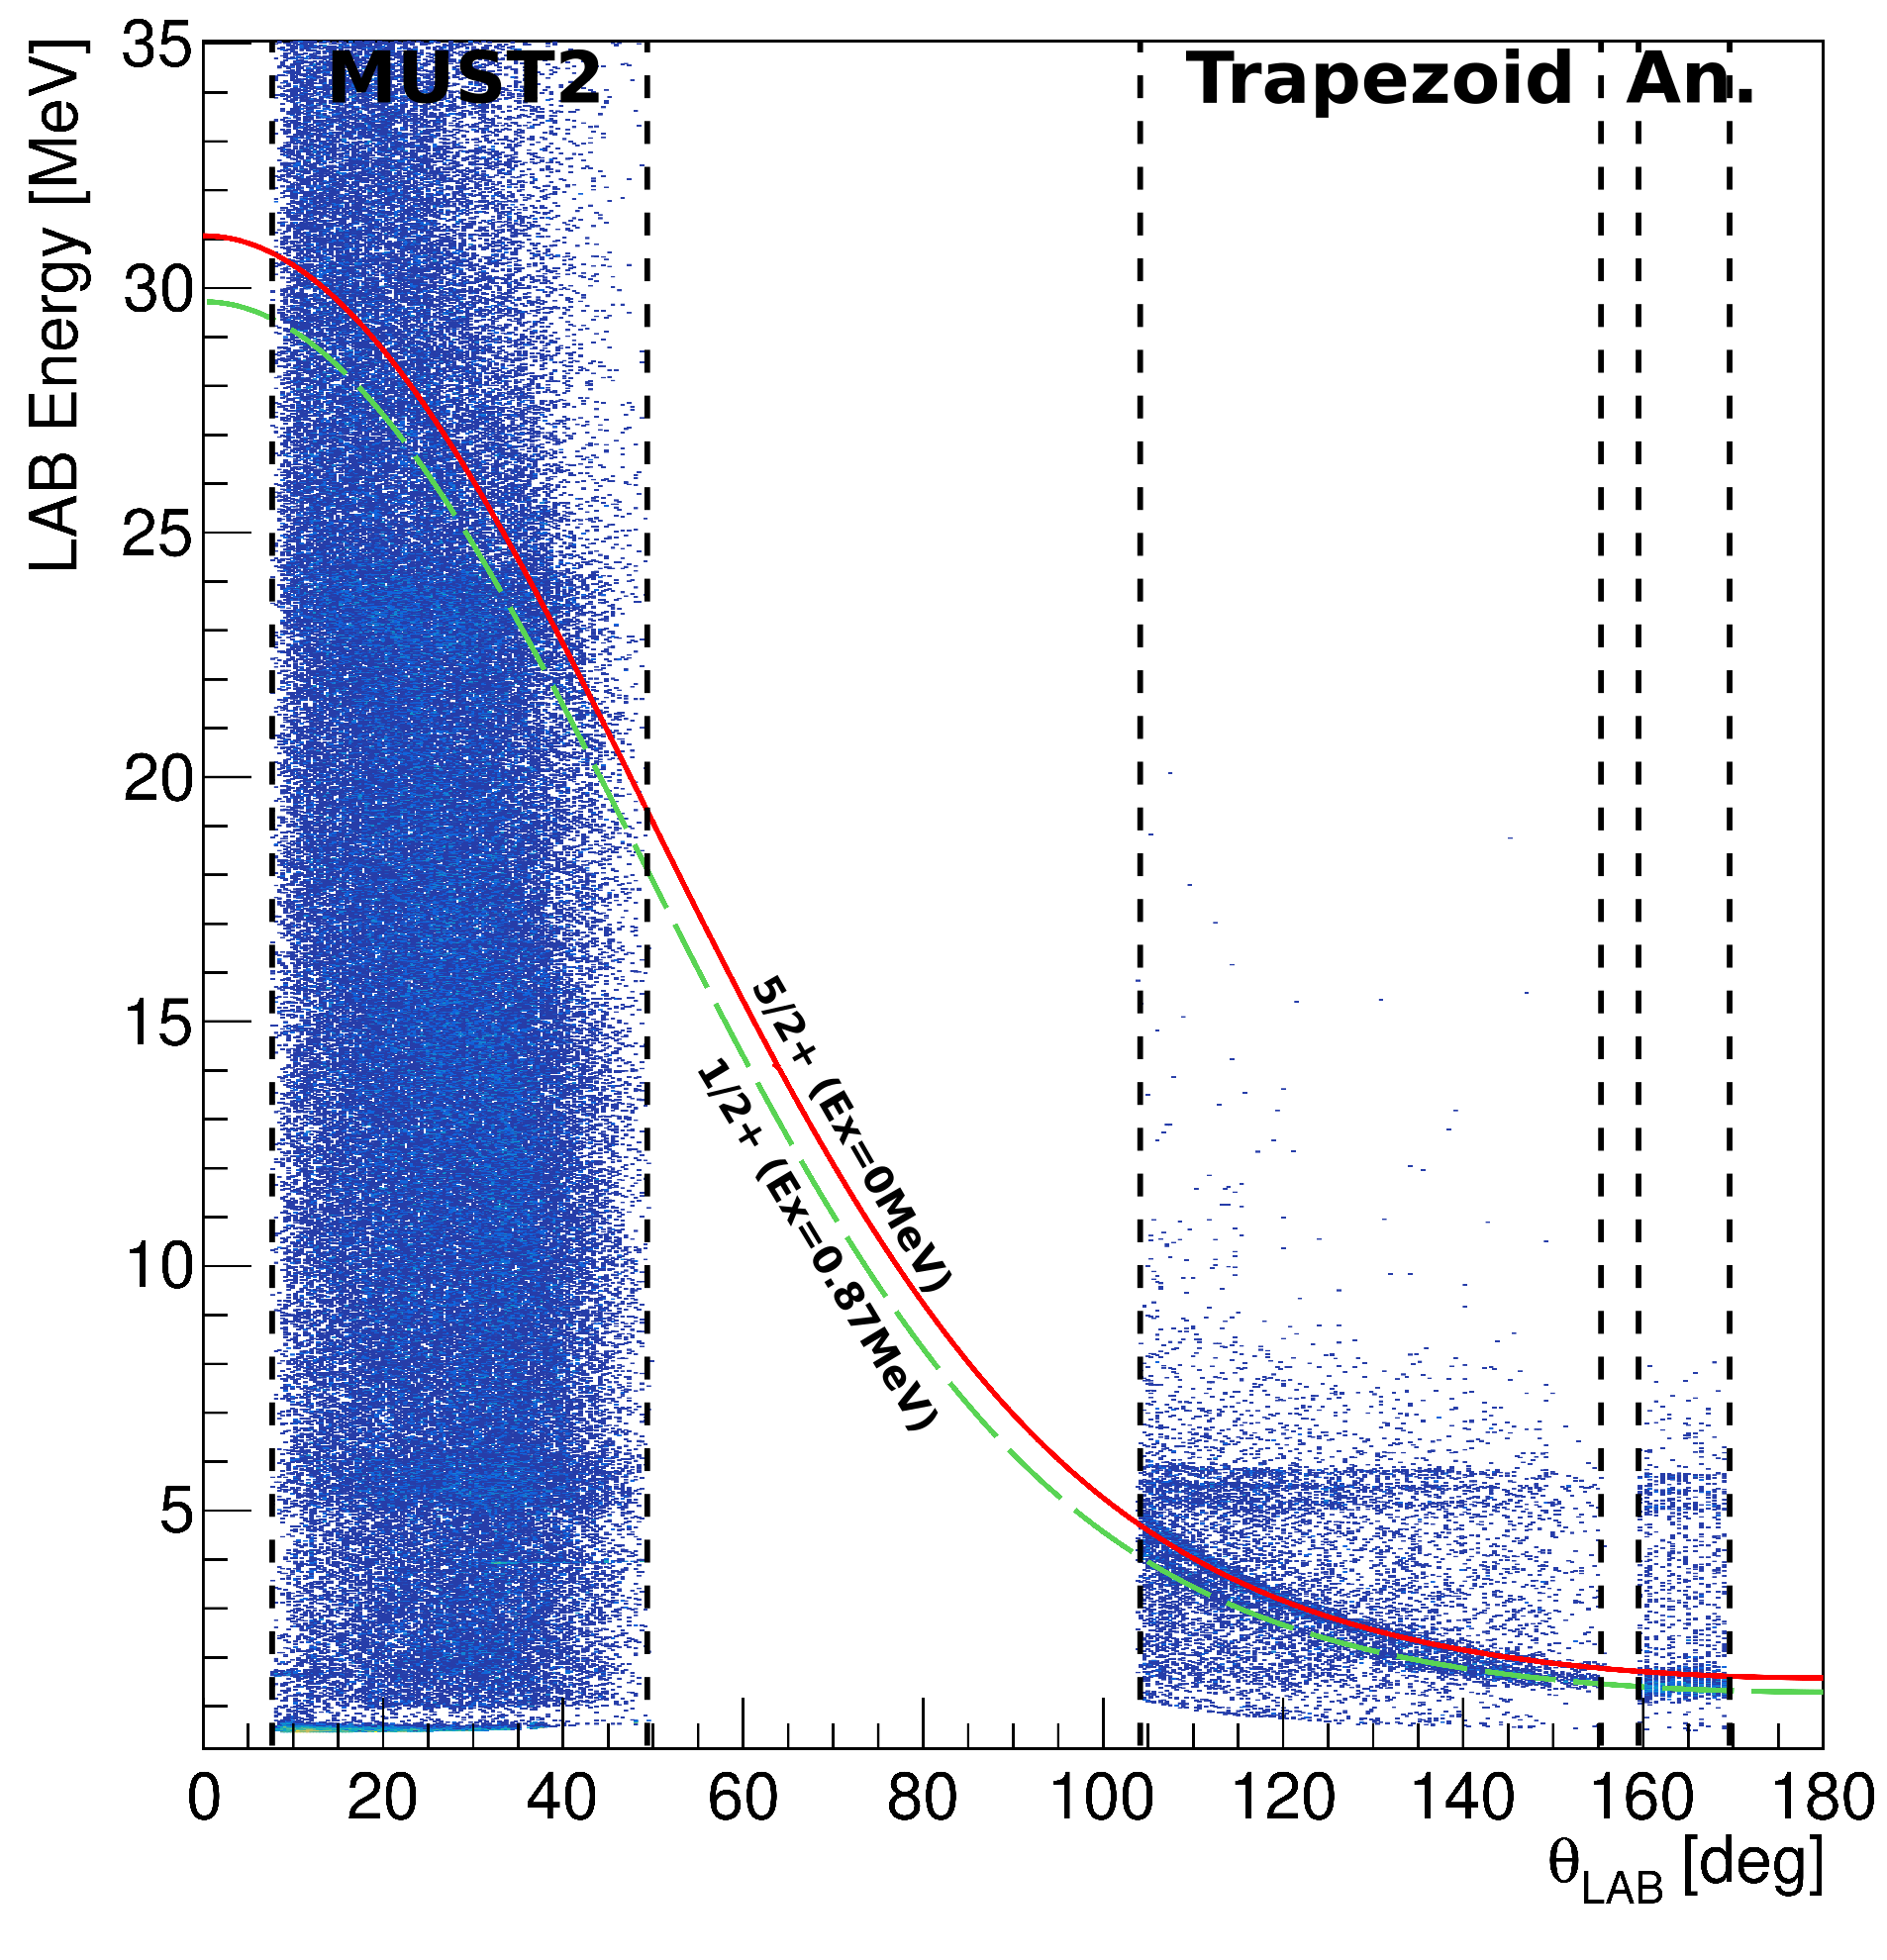
\includegraphics[width=1.14\textwidth]{ELabVsThetaLab_0.png}}
				\only<2>{\footnotesize Selection of particle only on Mugast\\
				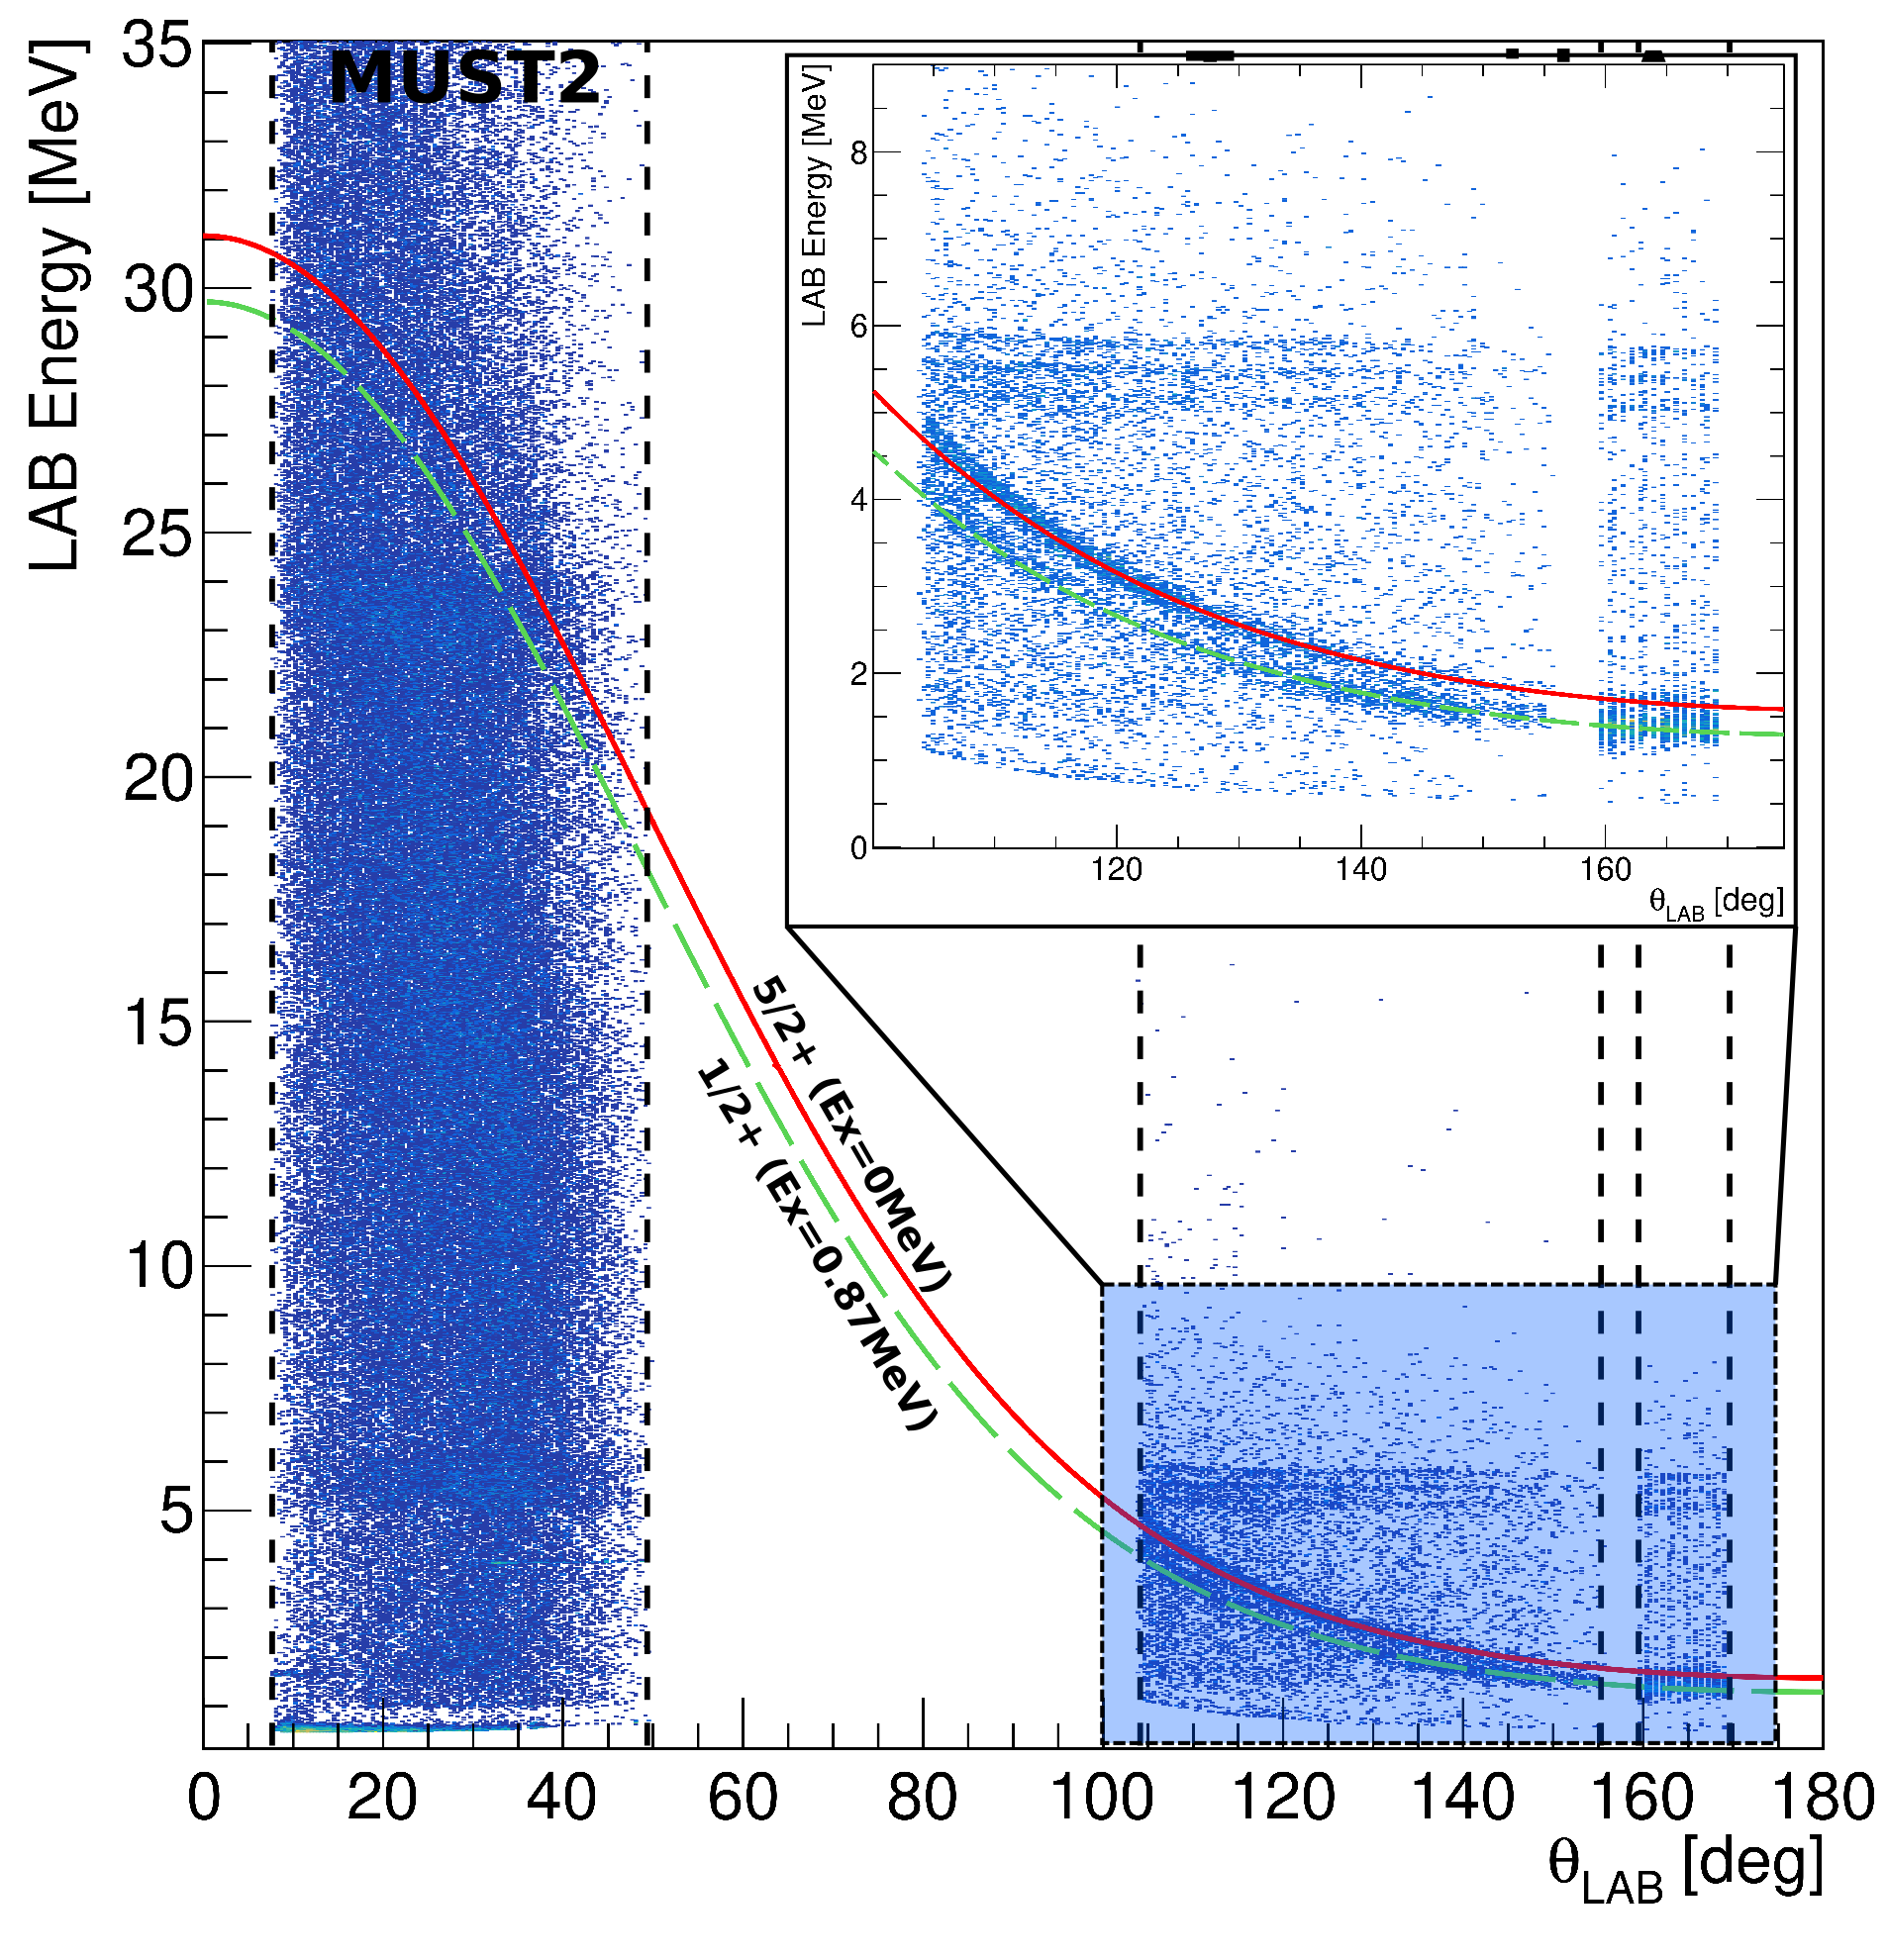
\includegraphics[width=1.14\textwidth]{ELabVsThetaLab_1.png}}
			\end{overlayarea}
		\end{column}
		\begin{column}{0.57\textwidth}
			\begin{overlayarea}{\textwidth}{\textheight}
				\centering       
				\only<1>{\footnotesize Excitation Energy\\
				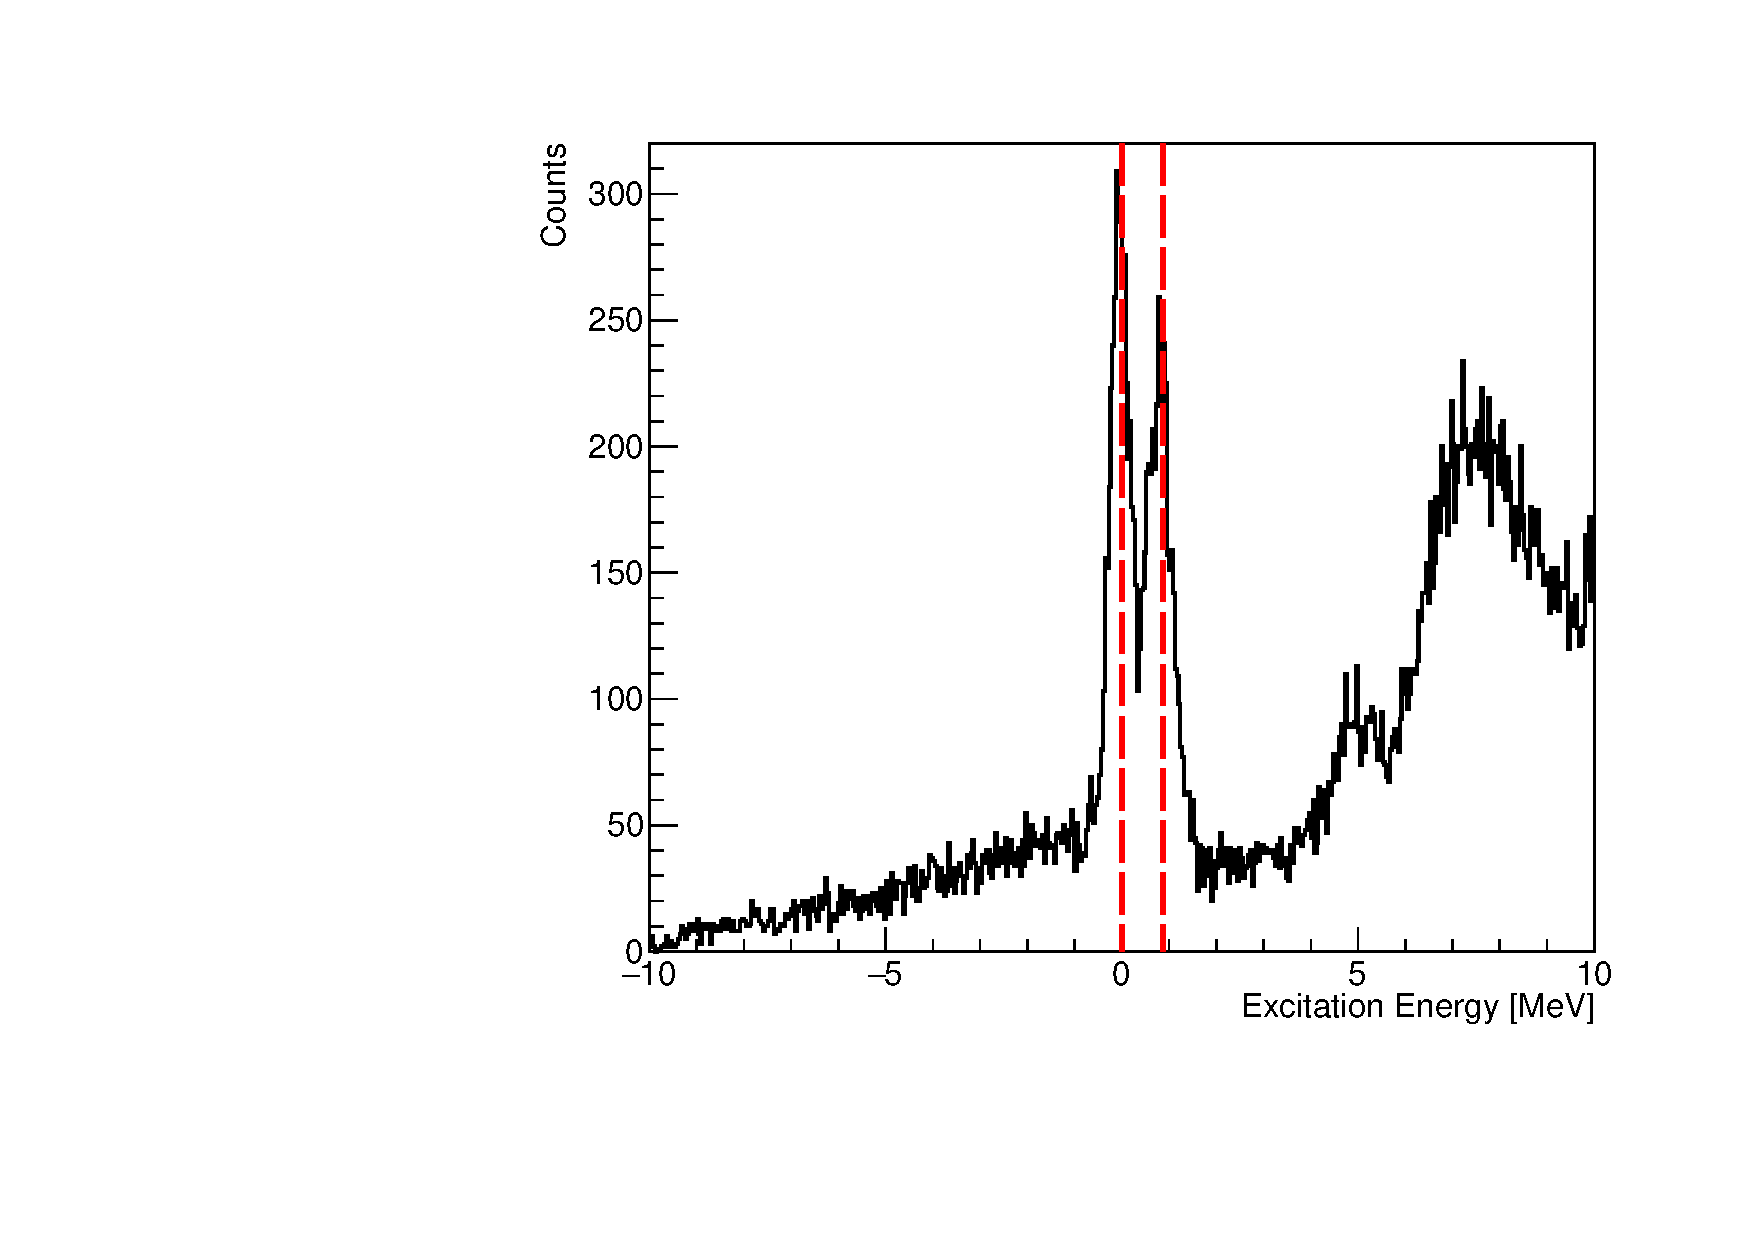
\includegraphics[width=1.05\textwidth]{Ex_0}}		
				\only<2>{\footnotesize Excitation Energy\\
				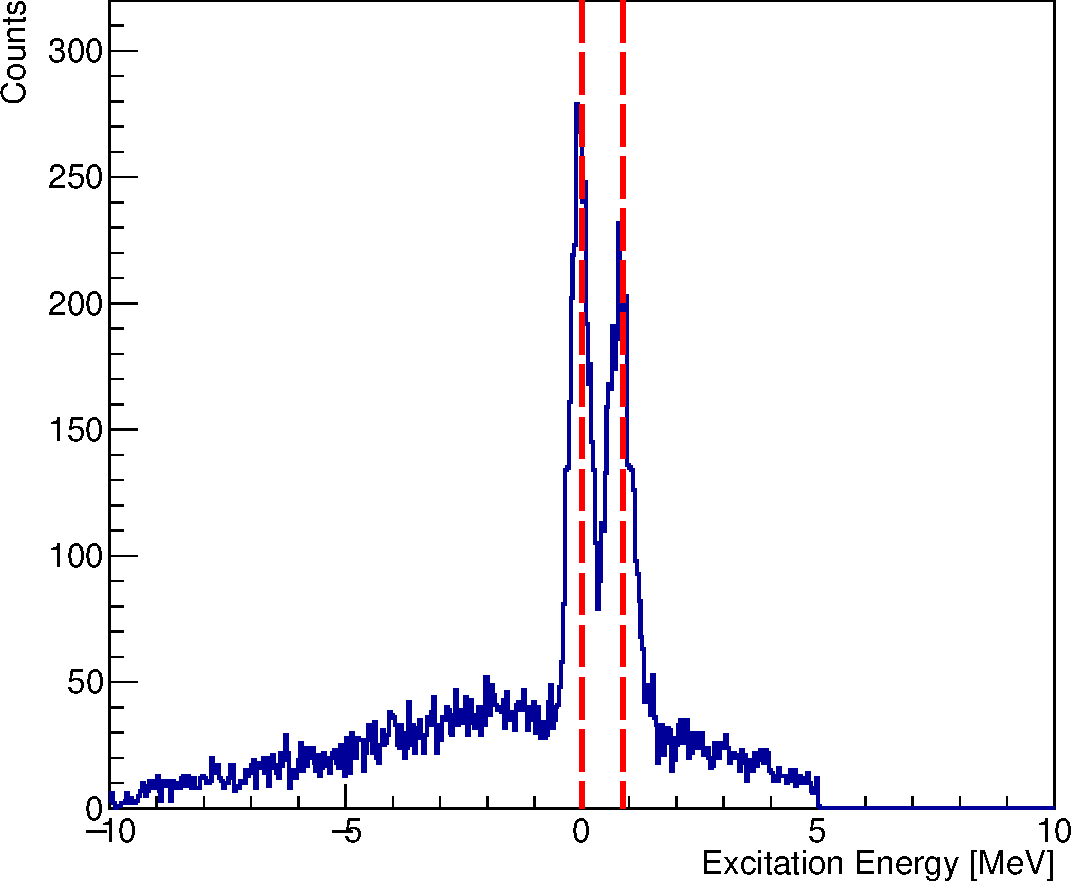
\includegraphics[width=1.05\textwidth]{Ex_1}}
		    \end{overlayarea}
		\end{column}
	\end{columns}
\end{frame}

\begin{frame}{Angular Distribution}
    	\vspace{-0.05\textheight}
    \begin{overlayarea}{\textwidth}{0.1\textheight}
	\centering
	\end{overlayarea}	
	\vspace{-0.05\textheight}
	\begin{columns}
		\begin{column}{0.43\textwidth}
			\begin{overlayarea}{\textwidth}{\textheight}
				\centering
				\vspace{0.02\textheight}
				\only<1>{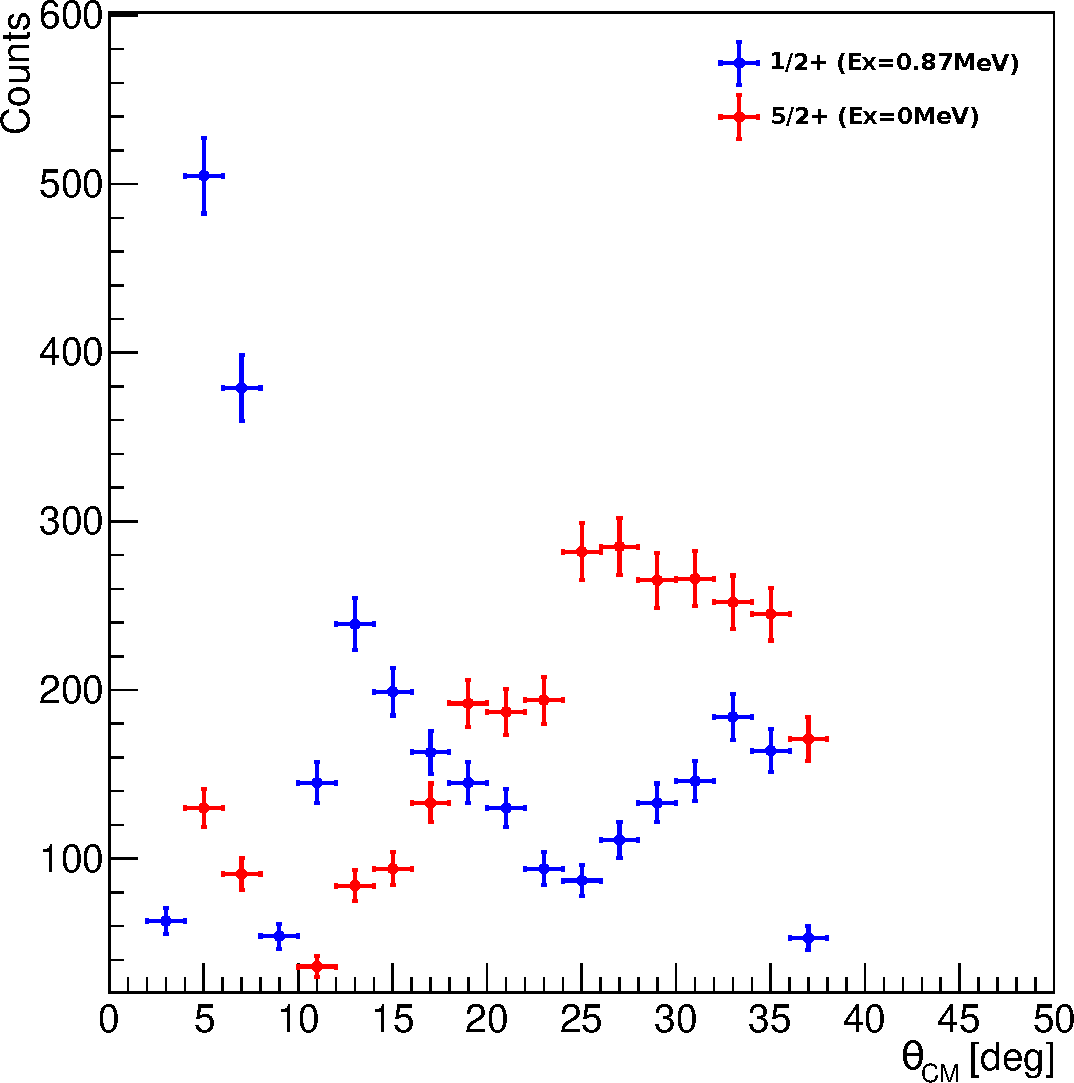
\includegraphics[width=1.09\textwidth]{ARawDist}}
			\end{overlayarea}
		\end{column}
		\begin{column}{0.57\textwidth}
			\begin{overlayarea}{\textwidth}{\textheight}
				\centering       
				\only<1>{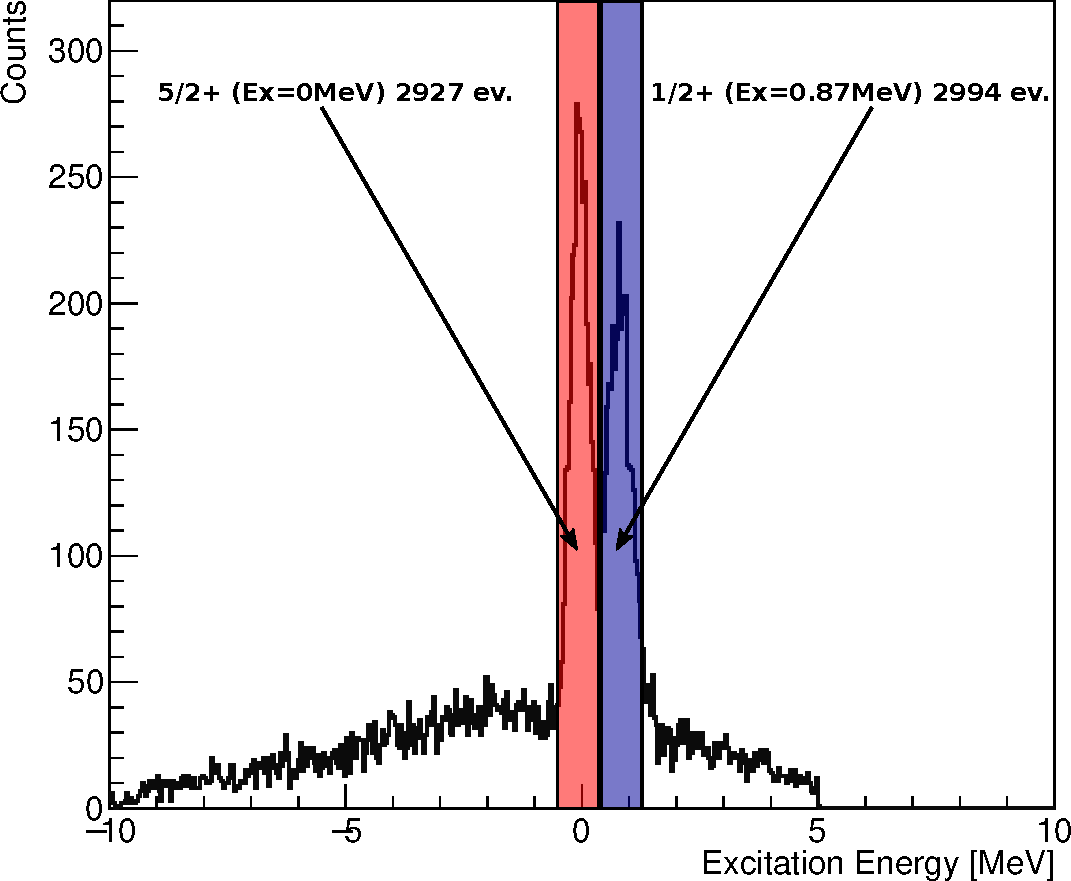
\includegraphics[width=1.1\textwidth]{Ex_2}}	
		    \end{overlayarea}
		\end{column}
	\end{columns}
\end{frame}

\begin{frame}{Differential Cross Section}
    	\vspace{-0.05\textheight}
    \begin{overlayarea}{\textwidth}{0.1\textheight}
	\centering
	\end{overlayarea}	
	\vspace{-0.08\textheight}
	\begin{columns}
		\begin{column}{0.4\textwidth}
			\begin{overlayarea}{\textwidth}{\textheight}
				\centering
				%\vspace{0.2\textheight}
				Normalized with simulated\\ angular efficiency\\
				$\downarrow$\\
				Fit over the theoretical\\ distribution\\
				\vspace{0.05\textheight}
				Efficiency normalization obtained from alpha source to be checked\\
				\vspace{0.05\textheight}

				\tiny DWBA calculation from Jesus Casal\\
				Università degli Studi di Padova\\
				INFN Sezione di Padova\\				
				\vspace{0.02\textheight}
				Optical potential from\\ An et al.,PRC 73.5 (2006)\\
				Watson et al., PR 182.4 (1969)\\
				 
			\end{overlayarea}
		\end{column}
		\begin{column}{0.6\textwidth}
			\begin{overlayarea}{\textwidth}{\textheight}
				\centering      
				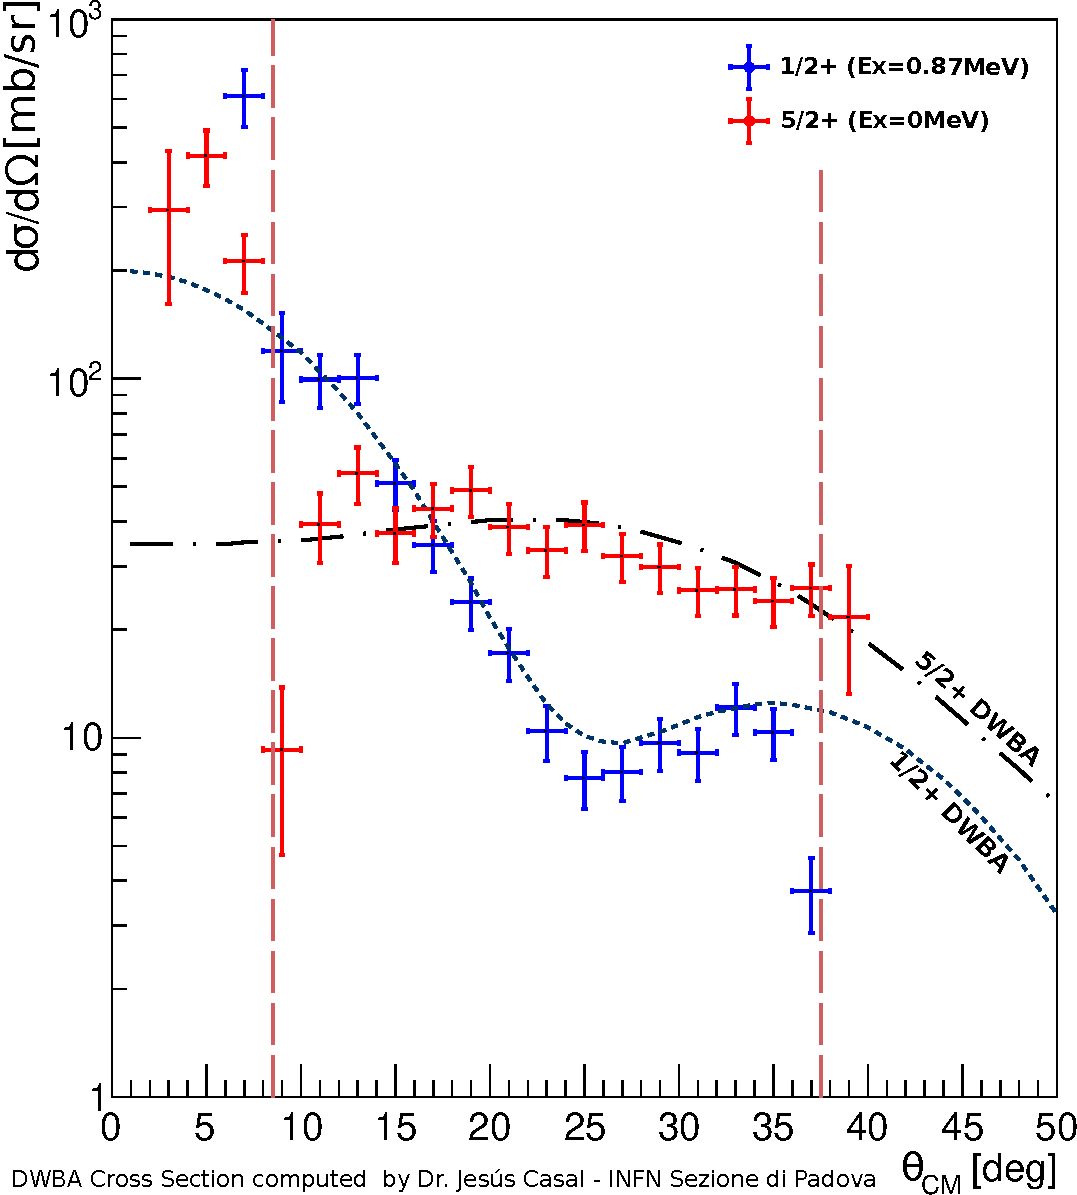
\includegraphics[width=0.9\textwidth]{ADist_jesus}			 				
		    \end{overlayarea}	
		\end{column}
	\end{columns}
\end{frame}


